\chapter{Background} \label{chp:background}

    In recent years, the commercialization of space has greatly captured the public's imagination. Access to low Earth orbit has been made much cheaper by new private companies. To access objectives deeper in space, including rapid transit of humans to Mars, the development of novel propulsion technologies is necessary. 
    
    The concept of laser-thermal propulsion (LTP) was first suggested by \textcite{kantrowitzRelevanceSpace1971} as a way to decrease launch costs and continues to be of interest. This method of propulsion uses a ground- or space-based laser to heat a gas on a spacecraft, which is then expelled out of a nozzle to generate the required thrust.

    In a conventional chemical rocket engine, the energy source is the oxidizer and the fuel, which are reacted together to release energy. They are transported with the rocket and set the temperature of the combustion reaction (typically \qtyrange{2000}{3000}{K}), which is proportional to the exhaust velocity.

    [Image to show what I mean (compare chemical to LTP rocket)]
    
    Separating the propulsion power source (here, the laser) from the spacecraft itself allows crucial weight savings, either increasing the payload mass fraction or decreasing transit time. Using a laser also allows for much higher thrust chamber temperatures than chemical propulsion, as the temperature of these plasmas is typically \qtyrange{15000}{20000}{K}. This gives in turn higher exhaust velocities. This propulsion method could therefore be an order of magnitude more efficient than our current rocket engines. To be practical for space propulsion, the main engineering challenges that need to be solved are:

    \begin{enumerate}
        \item Building a ground-based laser array powerful and precise enough to beam into orbit
        \item Increasing thermal efficiency
    \end{enumerate}

    This thesis will focus on the second challenge, as well as constructing a proof of concept 
    
    % , if certain engineering problems can be solved. The main question that remains is how to absorb as much laser energy as possible 
    
    %Russian work: 1960s-2000s?

    The experimental basis of this means of propulsion was developed by \textcite{generalovContinuousOpticalDischarge1970} in 1970. For the first time, an LSP was generated with a \qty{10.6}{μm} CW \ce{CO2} \qty{150}{W} laser. In this case, the LSP was ignited by a second, \qty{10}{kW} pulsed \ce{CO2} laser.
    
    Most studies have used CO2 lasers with a wavelength of 10.6 μm [3] - [6]. However, these concepts were limited by a short focusing range due to their long laser wavelength. 
    
    High power fiber lasers emitting near 1 μm (thus, having longer range) have recently become readily available, making laser propulsion more feasible than ever [7].

    
    %American work: 1970s-1990s?

        Work was done under a NASA grant in the 1970s by REF[Shoji and Larson] to design an LTP engine. 

    %Japanese work: 1980s-2020s?

        In the early 2000s, \textcite{toyodaThrustPerformanceCW2002} 
        
        \begin{figure}[h]
            \centering
            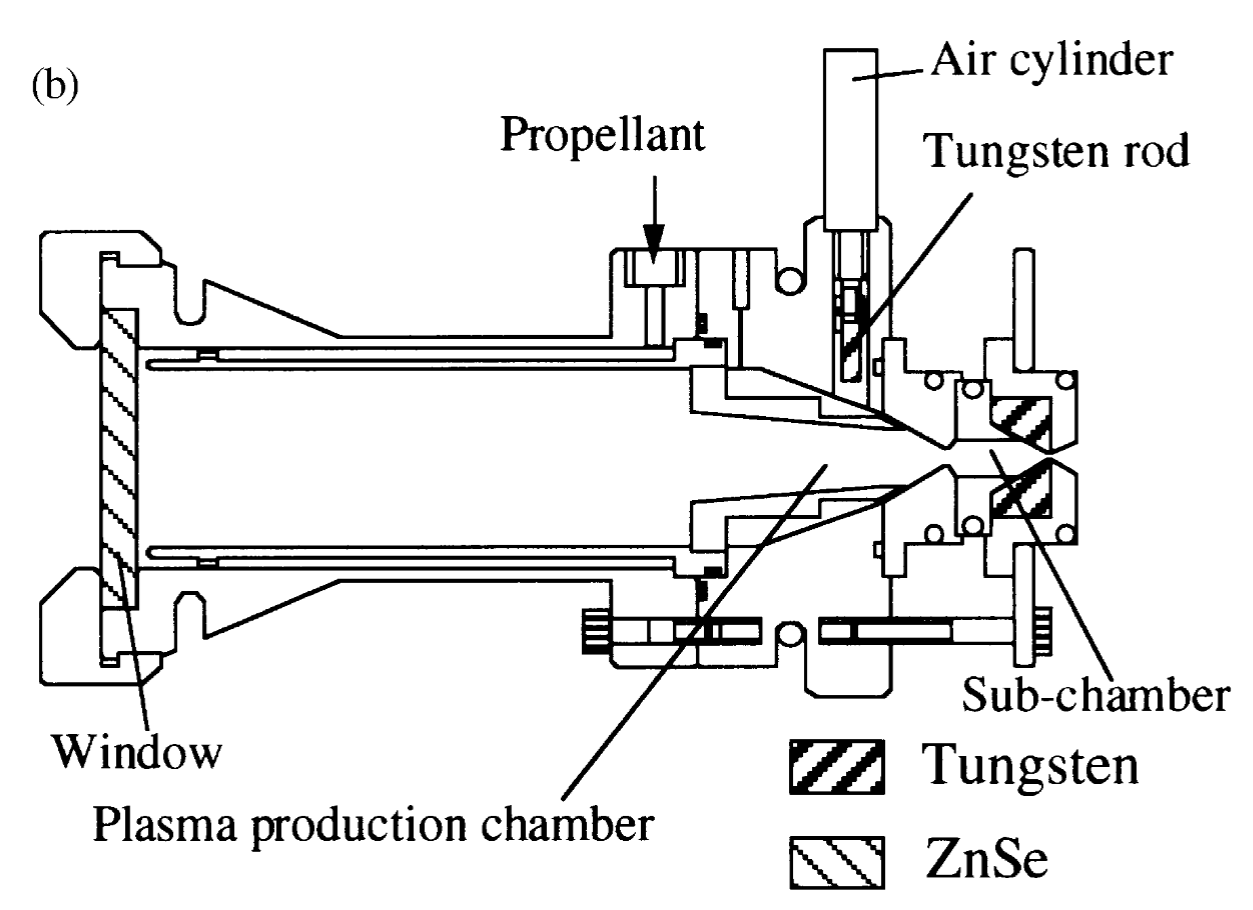
\includegraphics[width=0.35\textwidth]{assets/2 background/Toyoda Apparatus.png}
            \caption{Model II experimental apparatus from \textcite{toyodaThrustPerformanceCW2002}}
            \label{fig:Toyoda apparatus}
        \end{figure}

        More recently, work by Matsui [look into his work here https://scholar.google.com/citations?view_op=list_works&hl=fr&hl=fr&user=eeEONzQAAAAJ&sortby=pubdate]

    %Chinese work: 2020s?

        \textcite{luCharacteristicDiagnosticsLaserStabilized2022a} 

    %Canadian work: 2020s

        This thesis builds directly upon \textcite{duplayArgonLaserPlasmaThruster2024a}'s Master's thesis. 

    \section{Energy deposition}

        
        Increasing the amount of energy deposited by the laser into the working gas remains a topic of active research and is a significant hurdle for the operational use of LTP.

        % Graph of energy loss here (similar but not exactly same as Emmanuel's)

        The two main conversion efficiencies are:
        \begin{enumerate}
            \item Absorption of the laser energy by the plasma
            \item Heat transfer from the plasma to the working gas
        \end{enumerate}

        There is a problem when comparing efficencies , as the definition of efficencies are different from source to source. (Ex: Toyoda, Matsui, )

        Much work on the topic was done in the 1980s. \textcite{keeferPowerAbsorptionLasersustained1986a} studied LSP in a forced convective flow environment. Using a \qty{1.5}{kW} \ce{CO2} laser with power levels of \qtyrange{360}{840}{W} and pressures of \qtyrange{1.3}{2.3}{atm}, with varying flow velocities, the temperature field of the plasma was measured. From the temperature field, and assuming local thermodynamic equilibrium, the power absorbed by the plasma and the power radiated from it can be calculated.

        \begin{figure}[h]
            \centering
            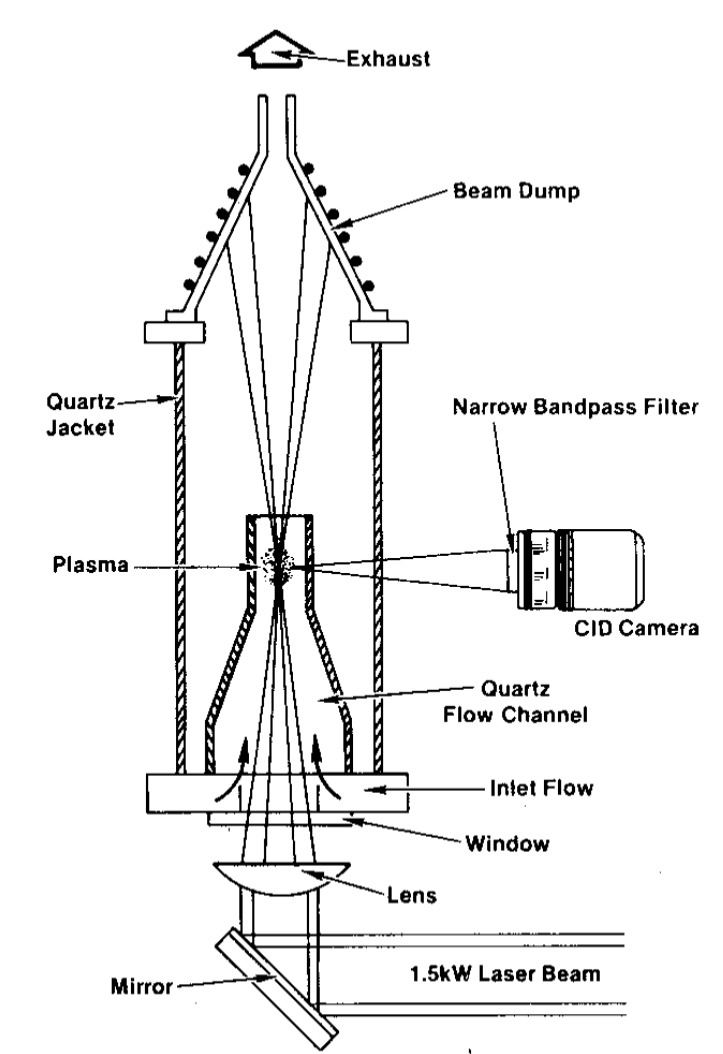
\includegraphics[width=0.35\textwidth]{assets/2 background/UTSI (Keefer) Apparatus.png}
            \caption{Experimental apparatus from \textcite{keeferPowerAbsorptionLasersustained1986a}}
            \label{fig:Keefer apparatus}
        \end{figure}
        
        \autoref{fig:Keefer apparatus} shows the apparatus used for these measurements. An inner quartz flow channel contains the plasma, while an outer quartz jacket contains the pressure. Flowing argon comes in from the bottom and into the flow channel. The plasma is initiated by laser heating of a tungsten rod, which was removed after ignition. Downstream, a water-cooled copper beam dump absorbs the laser energy and cools the heated argon flow.

        \Citeauthor{keeferPowerAbsorptionLasersustained1986a} determined that % PUT PERCENTAGES HERE

        In parallel, a group from the University of Illinois (say this differently?), claims absorption approaching \qty{80}{\%} and thermal efficiency

        \begin{figure}[h]
            \centering
            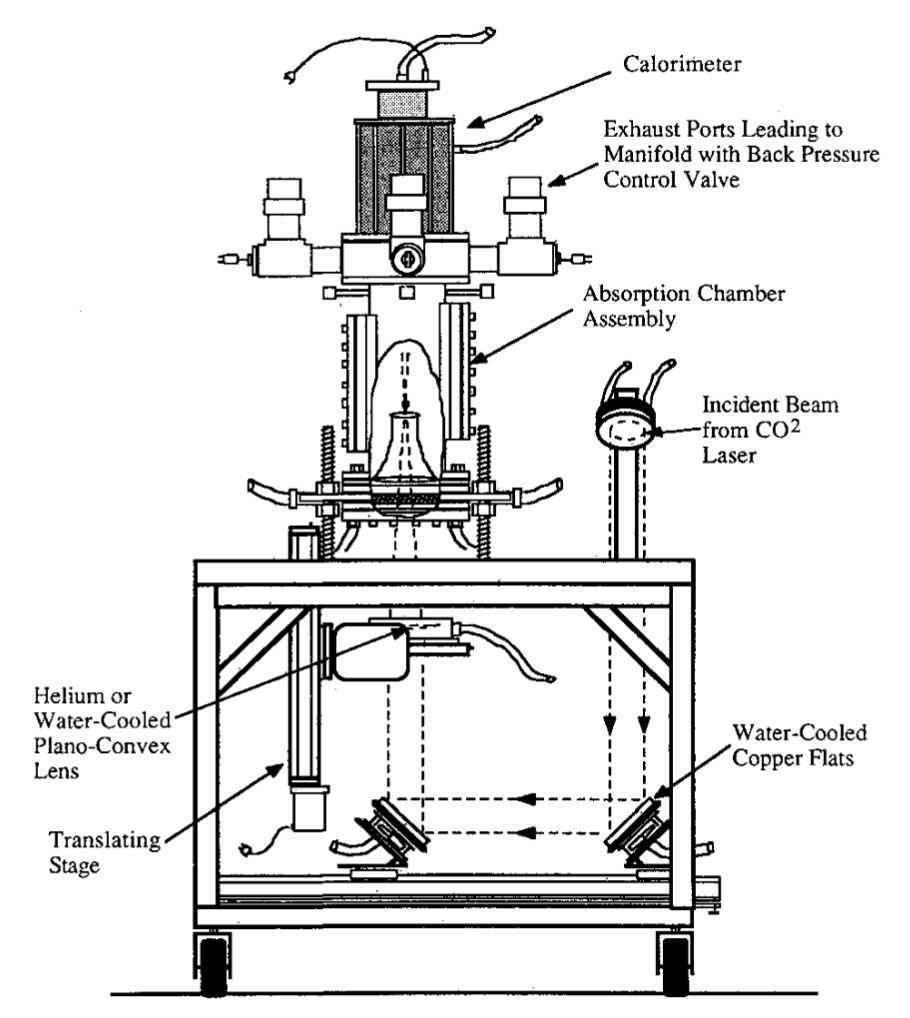
\includegraphics[width=0.35\textwidth]{assets/2 background/Illinois (Krier) Apparatus.png}
            \caption{Experimental apparatus from \textcite{zerkleLasersustainedArgonPlasmas1990}}
            \label{fig:Krier apparatus}
        \end{figure}

        In their later work in 1990, \textcite{zerkleLasersustainedArgonPlasmas1990}, claims absorption from \qtyrange{55}{97}{\%} and thermal efficiency from \qtyrange{11}{46}{\%}. %continue this review, define "thermal efficiency"

        %LTP research slowed down with the end of high-power laser weapon research in the early 1990s.

        Thrusters with higher laser powers were experimented with by \textcite{blackLaserPropulsion10kW1995}, with a \qty{10}{kW} \ce{CO2} laser. Both argon and hydrogen were used.

        In this study, a preliminary design for a \qty{100}{kW} thruster was presented, with a predicted specific impulse of \qty{1000}{s}, thrust of \qty{4.5}{N} and a conversion efficiency of \qty{80}{\%}.

       

        

        % Lubin papers

        % To change/update: Preliminary work done by the McGill Interstellar Flight Experimental Research Group indicated that with the first generation thruster, about \qty{80}{\%} of the laser energy was being absorbed by the plasma, with approximately \qty{15}{\%}

    \section{Seeding}

        Seeding the working gas with another species has been discussed as a way to increase the efficiency of an LTP engine.

        Carbon particles are a candidate explored by many papers. %Which ones?

        Pure methane and methane-seeded xenon have been experimentally investigated by \textcite{kameiMethaneMethaneXenon2020}. % What are conclusions of this? 
        The rationale is similar to carbon particles, as the methane dissociates into hydrogen and carbon with the high temperature of the LSP.

    \section{Summary and direction of work in this thesis}

        \begin{table}[ht] % TODO - update this table
            \small
            \centering
            \caption{Summary of a selection of past LSP experiments. $\lambda$: wavelength, $P$: maximum laser power, $p$: pressure, $I_\mathrm{sp}$: maximum specific impulse, $F_\mathrm{T}$: maximum thrust}
            \label{tab:pastexp}
            \begin{tabularx}{\textwidth}{@{}>{\small}X<{\raggedright}llrrlrrr>{\footnotesize}X<{\raggedright}@{}}
            \toprule
            {LSP   Facility}                                                           & Year & Laser         & $\lambda$   [\unit{\um}] & $P$ [kW] & Gas                 & $p$   [atm] & $I_\mathrm{sp}$ [s] & $F_\mathrm{T}$   [N] & {Comments}                                                                   \\ \midrule
            \textcite{generalovContinuousOpticalDischarge1970}                                                         & 1970 & \ce{CO_2}                  & 10.60             & 0.15               & \ce{Xe}              & 3.0 - 4.0        &           -             &       -       & First   LSP                                                                \\
            \textcite{keeferPowerAbsorptionLasersustained1986a}         & 1986 & \ce{CO_2}                  & 10.60             & 0.84        & \ce{Ar}              & 1.3   - 2.3      &            -            &       -       & Specialized   laser beam dump integrated within the converging exit nozzle \\
            \textcite{blackLaserPropulsion10kW1995}          & 1995 & \ce{CO_2}                  & 10.60             & 10.00              & \ce{Ar},   \ce{H_2}    & 1.0   - 2.7      & 350                    & 3.00         & 15:1   expansion ratio nozzle                                              \\
            \\
            \textcite{toyodaThrustPerformanceCW2002} & 2002 & \ce{CO_2}                  & 10.60             & 2.00               & \ce{Ar},   \ce{N_2}    & 2.0   - 5.5      & 113             & 0.44         & Tungsten   rod ignition                                                    \\
            \textcite{zimakovInteractionNearIRLaser2016}                                                        & 2016 & Fiber                & 1.07              & 1.50        & \ce{Ar},   \ce{Xe}   & 3.0   - 24.7     & -                      & -            & Arc   discharge ignition                                                   \\
            \textcite{matsuiGeneratingConditionsArgon2019}                                                          & 2019 & Fiber &      1.07             &        2.00            &           \ce{Ar}           &          1.0 - 64.2        &            -            &       -       & Arc   discharge ignition                                                   \\
            \textcite{luCharacteristicDiagnosticsLaserStabilized2022a}                                                             & 2022 & Fiber                & 1.08              & 0.30      & \ce{Ar},   \ce{Ar + N_2} & 9.9   - 19.7     & -                      & -            & Arc   discharge ignition                                                   \\ \bottomrule
            \end{tabularx}
        \end{table}

        % Higgins text from email to Mark Wolverton: Laser thermal propulsion originated with Arthur Kantrowitz, who was involved in developing the first gas dynamic lasers that would be able to reach MW-class power in the 1960s. (Interesting connection to Jordin Kare: Jordin was also a filk-singer, which is a science-fiction themed version of folk singing. He actually wrote a song about laser thermal propulsion called “Kantrowitz 1972”. Put your coffee cup down before listening to this…) 
        %The laser-thermal rocket kind of died with the demise of high-power laser weapon research in the early 1990s. Now with Phil Lubin’s work, I think it is worthwhile looking at again. Even with a gigawatt-class laser, laser propulsion is not well suited for ground-to-orbit launch vehicles, unless they are very small (this is what Jordin’s filk song is about—rapid turn around of launching many microlaunchers using a laser).  Here’s the clip of Elon Musk making the same point: https://youtu.be/viRylmoFAj0?si=MzzsBkhHF71FLCRG
        
        %However, with Philip Lubin’s demonstration that phased array lasers can be made arbitrarily large, we can now reach much deeper into space and perform propulsive maneuvers more leisurely (say, over hours), so the power requirements now drop to the 100s of MW (rather than 10s of gigawatts!). This was the basis of our 45-days-to-Mars study, which I think you have already seen. Here is an un-paywalled version of it: [2201.00244] Design of a rapid transit to Mars mission using laser-thermal propulsion (arxiv.org)

        %The other approach is to provide laser power onto a solar panel (although one tuned to the laser wavelength) that then powers electric propulsion like an ion engine or Hall effect thruster: Laser-electric propulsion. Lubin’s group published a similar study to ours, trying to hit similar objectives (the usual “Mars in a month” metrics). I’ve attached their paper here: SheerinLubinEtAl_FastTransporationElectricPropulsionDirectedEnergy_ActaAstro2021
        %Their paper and ours make for a nice “compare and contrast” of the pluses and minuses of the laser-electric and laser-thermal approaches.

        \section{Objective}

            The objective of this research project is to test a lab-scale proof-of-concept LTP thruster for interplanetary space flight, using a \qty{1.07}{um} fiber laser. The main objective of the proposed research will be to measure the key performance parameters of this thruster (thrust and specific impulse notably), as well as characterize the laser-sustained plasma (LSP) heating core inside the thruster. This project will validate theoretical insights recently developed by the McGill Interstellar Flight Experimental Research Group \cite{baoTwoDimensionalSimulationLaser}, \cite{duplayDesignRapidTransit2022a} and continue the experimental research started by \textcite{duplayArgonLaserPlasmaThruster2024a}. % Plus, add "Determine the effect of seeding on thrust performance"

            % mention The original contribution of this work ?
